\chapter{Experiments Design}
\label{chap:Evaluation}
This thesis work introduces software development stream and micro-process
to study software development process. Adoption and learning curves of best
practice in software development impair process development as well as best
practice evaluation. SDSA framework aims at improving both experimental
evaluation and practical execution of best practice in software development
by recognizing micro-process and quantifying best practice execution. 

We will undertake two separated experiments to study correctness and
effectiveness of SDSA in software development best practice evaluation.  In
our study we choose best practice Test-Driven Development as the bechmark
to evaluate our SDSA framework. As a well-known best practice welcomed by
many developers, Test-Driven Development defines two simple rules only such
that experiment subjects can comprehend it easily. Experiment one is best
practice micro-process discovery and validation. The goal of this
experiment is to evaluate how good SDSA can understand development process
and best practice execution. It sets up the benchmark on how system performs
to identify best practice and what kind violations it may detect. In experiment 
two we will use SDSA on a controlled experiment of Test-Driven Development. The
controlled experiment will be the replication of already done experiment on
Test-Driven Development in other organizations. The SDSA-powered experiment
is expected to reveal more detailed information on how test subjects performs
instead vaguely assuming best practices are there. 

\section{Software Development Stream Analysis Framework Validation}
Automatic data collection, development stream contruction, episode
tokenization and micro-process classification are four basic elements of
SDSA framework. This experiment is to test whether it can tell the
difference when developer execute the best practice and when they do not.
Because experiment subjects may or may not have enough skills to write unit
tests, not even to test first we will ask test subjects work on three
problems to build and exercise Test-Driven Development skills. Task 1 is a
simple programming task for us to understand test subject's development
skills, developers should only spend 20 to 40 minutes to finish without
experiment observer's assistance. An optional introduction of unit test
will be provided before subjects work on second experiment. As an
additional requirement we ask all test subject to produce more than 90\%
statement coverage. Experiment assistants will provide technique support to
help test subjects achive high coverage. The coverage is evaluated with
Clover. We will introduce Test-Driven Development before problem 3 and ask
test subjects to work on it following best practice Test-Driven
Development. Similarly as previous experiment we ask for 90\% above
statement coverage too in this experiment.

\subsubsection{Objectives}
Fine tune the development stream construction, episode tokenization and
micro-process classification to measure Test-Driven Development precisely
and differentiate development process quantitatively with SDSA framework.

\subsubsection{Elements of Experiments}
\begin{enumerate}
\item \emph{Subjects} Test subjects are undergraduates who have finished
  one or two 300 level classes already and graduate students. Knowing Java
  and good understanding of Object-Oriented Programming are two basic skills
  required.
\item \emph{Problem Sets} 
  \begin{description} 
  \item Problem 1 is a movie listing management system.  It should be able
    to add a move, delete a movie, modify a move and print out list of all
    movies. Database usage is prohibited for the sake of simplicity and
    user interface is via DOS command line input. It is optional to have
    unit tests. (Approx 20-40 min)
  \item Problem 2 is a stack data structure implementation. Elements in the
    stack are integer objects only. Implemention of stack must be in
    object-oriented style and it test coverage has to be at least 90\%.
    (Approx 20 min)
  \item Problem 3 is a bowling score system. It should tell the correct
    score given a set of bowling throws. We require test subjects write
    programs in Test-Driven Development fashion, and statement coverage
    must reach 90\% at least. In the mean time we want to observe how
    developers conduct Test-Driven Development. Observes will record down
    Test-Driven cycles and violation of Test-Driven Development. We will
    look for an alternative solution to record development process without
    disturbing development work.
  \end{description}
  
\item \emph{Development Tools} Eclipse IDE is the only developement we will
  use in the entire development process. Although Eclipse experience is a
  plus we don't require test subject know Eclipse well to increase our
  chance to recurit approachable test subjects. Development environment
  will be set up by examiners beforehand and we only ask subjects do simple
  tasks only.
\item \emph{Observer and Recorder} It is unsure whethere SDSA framwork can
  canonically reflect development process in the context of Test-Driven
  Development such that we include oberver role in our experiments.
  Observers must know Eclipse well and understand Test-Driven Development
  well. Upon request observers should be able to answer possibly
  sophisicated unit test and Test-Driven Development question. An a
  complement tool we may also monitor and record the development process
  without interfereing test subjects' development process. 
\item \emph{Pre-experiment Survey} Purpose of this experiment is to verify
  SDSA framework implementation so we want diverse test subject population.
  We will include undergraduate, graduate, and possiblely professional
  developers in our experiment. The pre-experiment is informational about
  test subjects.
\item \emph{Post-experiment Survey} Mostly it will be about the test
  subjects' understanding of Test-Driven Development from experiments. 
\end{enumerate}

\subsubsection{Experiment Setup and Procedure}
\subsubsection{Result Analysis}

\section{Evaluation of Test-Driven Development with Assistenance of SDSA framework}
Our motivation to development SDSA framwork is to provide a generic
framework to help best practice practitioners to undertake experiment and
evaluation effectively. Delicate best pracice such as Test-Driven
Development requires high discipline on test subjects, which is hard and
expensive to be managed. The light-weight framework of SDSA powered by
Hackystat will provide in-process development process data. We will replicate
Test-Driven Developments experiments in our study to validate the arguments
contradicted by previous studies.

In the classroom setting we will randomly assign student in the class into
two different groups. They will have the same lecture and teaching
materials.  We require everybody must reach 90\% cover coverage at least.
Group one students has the option to test-last or follow the traditional
water-process. Group 2 students are asked to do Test-Driven Development. In
order to improve the execution effectiveness we ask developer to write a
well-known stack application to improve the understanding of Test-Driven
Development via a tutorial session.

\begin{comment}

This work provides a test development viewer tool to quantatively analyze
Test-Driven Development process using in-process software metrics support.
It can tell whether developer do TDD or not and how unit tests are created
and exercised. In my thesis work I will exam following claims regarding to
TDD with this viewer tool:

\begin{enumerate}
\item 100\% execution of Test-Driven Development is not practical. More or
  less developers will do ad-hoc testing in development, that is to say,
  unit tests are written after implementation code exists.
  
\item TDD helps to yield higher quality code than ad-hoc unit testing and
  TLD. There are significant difference between TDD and TLD.

\item Because of high discipline requirement of TDD, most people will not
  stick to TDD or large portion of their code will not be implemented in TDD
  fashion even though they prefer to it.
\end{enumerate}


To evaluate these claims I propose a series of 5-stage experiments in software
engineering class in spring 2005.

\begin{enumerate}
\item {\bf Skills Building} At beginning of the semester students will
  learn advanced java development skills including Eclipse IDE, JUnit, ANT,
  Hackystat and so forth. They will work on some assignments to practice
  these skills. Hacksytat sensor for Eclipse will be installed as one
  requirement.
  
\item {\bf Project Inition} A semester-long project assignment will be
  given. Students can practice their design, development and unit testing
  skills.

\item {\bf Test-Driven Development} We introduce Test-Driven Development to
  students and ask them to do TDD in their projects. Students can use
  TDDViewer to check their development process.
  
\item {\bf Full-fledged Test-Driven Development} After last round students
  begin mastering TDD. They are required to work on their projects
  following TDD rationals in this iteration.

\item {\bf Post-TDD Adoption} At last step students are free to choose how
  they develop their projects. TDD is not a demand at all.
\end{enumerate}

With this experiment I will be able to test my hypotheses on Test-Driven
Development respectively as following.

\section{Claim 1: Test-Driven Development cannot be done stringently}
Test-Driven Development brings confidence on the code being developed and
also provides other benefits like clear design, robust code, 100\% test
coverage and development effort saving etc. if it can be done perfectly. In
practice this is not applicable even people believe they do TDD very well
in their development process. 

With the educational experiment I can test this by observing how much
portion work is being done in TDD at each iteration. Figure
\ref{fig:TDDTendency} is an example data I may get out of Test-Driven
Development experiment.

\begin{figure}[ht]
  \centering
  \includegraphics[width=0.5\textwidth]{figs/TDDPercentage.eps}
  \caption{TDD Percentage Tendancy}\label{fig:TDDTendency}
\end{figure}
  
This charts shows that more work is done under Test-Driven Development
rationals after students are familar with TDD. In addition to quantatively
telling how much percent work is done in TDD I will also do a survey too.
Appendix A lists the questionnaire to ask students' evaluation and
acceptance to Test-Driven development.

To evaluate this claim I need to supply a pilot implementation which is
done in 100\% TDD. Kent Beck's Cash Exchange example and his footage of
implementation will be used for calibration.

\section{Claim 2: Test-Driven Development yields higher code quality and costs less time}

Assumably Test-Driven Development yields high quality program. In the
experiment if students fail to do TDD well they are likely to produce low
quality code. To evaluate this claim I will collect development active
time, Test-Driven Development active time and code quality evaluation
including number of defects, test coverage and black-box test pass ratio.
Black-box tests are external tests. I will develop a series of black-box
tests to go through all projects to have external validation for code
quality.

Suppose there are 30 black-box tests. Following table contains number of
passed tests to each group. In the table a colum is number of passed tests
under each cateory. To each category average, maximum and minimum values
are listed.

\begin{table}[ht]
\centering
\caption{Number of Passed Tests}
\begin{tabular}{|c|c|c|c|c|} \hline
        &  \textless 50\% & 50-70\% & 70-85\% & 85-100\% \\ \hline
Average & 18 & 22 & 26 & 28 \\ \hline
Minimum & 10 & 15 & 21 & 25 \\ \hline
Maximum & 26 & 25 & 29 & 30 \\ \hline
\end{tabular}
\end{table}


Here block-box test is the proxy for code quality. To course projects,
grading is another proxy to project quality measure. Suppose 60\% out of
100 points will be given to project we may get following distribution.

\begin{table}[ht]
\centering
\caption{Grade v.s. TDD Percentage}
\begin{tabular}{|c|c|c|c|c|} \hline
        &  \textless 50\% & 50-70\% & 70-85\% & 85-100\% \\ \hline
Average & 36 & 44 & 51 & 55 \\ \hline
Minimum & 20 & 33 & 38 & 52 \\ \hline
Maximum & 52 & 51 & 62 & 61  \\ \hline
\end{tabular}
\end{table}

Test coverage will be referred but not a factor to determine code quality
because 100\% code quality can be achieved no matter test is written before
or after code implementation. But I will use test coverage to evaluate
Test-Driven Development because TDD should end with high test coverage even
100\%. Similarly test coverage can be as below.

\begin{table}[ht]
\centering
\caption{Code Coverage v.s. TDD percentage}
\begin{tabular}{|c|c|c|c|c|} \hline
        & \textless 50\% & 50-70\% & 70-85\% & 85-100\% \\ \hline
Average & 70\% & 80\% & 85\% & 90\% \\ \hline
Minimum & 66\% & 75\% & 77\% & 86\% \\ \hline
Maximum & 72\% & 90\% & 91\% & 100\%  \\ \hline
\end{tabular}
\end{table}

I will also look at the development time on test code and production code
to study how much time is spent on them respectively. Theoretically speaking
developers should not spend large amount of time on test code in the development.

\section{Claim 3: Discipline requirement hurdles Test-Driven Development adoption}

It is said developers can get ``test infected'' once they do Test-Driven
Development because of the incrediable confidence and other benefits TDD
brings to them. Once you get infected you will never go back to your old
development habits. It's an interesting issue to address because adoption
is always a problem for new technology. It is even harder for developers to
adopt TDD because it is counter-intuitive. In software development
education students are taught to cut down problems using top-down or
divide-and-conquere analysis skills. Traditionaly unit tests are conducted
by customers or test specialists. Unit testing is not a concern at all
untill Kent Beck came up with Test-Driven Development and xUnit framework.
I hypothesize that people will go back to their old development habits even
though they realize the benefits of Test-Driven Development.

In last iteration of experiment students can choose their development
methods as they want. My expection is that there will be a big drop of
Test-Driven Development percentage as shown in figure
\ref{fig:TDDTendency}. To study why student keep doing or abandon
Test-Driven Development I will conduct a survey to investigate it.


\end{comment}



















